\documentclass[12pt, letterpaper]{article}
\usepackage[left=1.00in, right=1.00in, top=1.00in, bottom=1.00in]{geometry}
\usepackage{amsmath}
%\usepackage{apacite}
\usepackage{graphicx}

\title{Chapter 2}
\author{Daniel C. Furr}
\date{\today}


\begin{document}

\newcommand{\genupsilonsq}{0.11} 
\newcommand{\gentau}[1][]{0.00, 0.10, 0.30, {#1} 0.50} 
\newcommand{\gentausq}[1][]{0.00, 0.01, 0.09, {#1} 0.25} 
\newcommand{\rsq}[1][]{0.30, 0.55, 0.92, {#1} 1.00} 
\newcommand{\aic}[1][]{7, 8, {#1} 9} 
\newcommand{\bic}[1][]{33.88, 38.72, {#1} 43.56} 
\newcommand{\nreps}{500} 
\newcommand{\nitems}{32} 
\newcommand{\npersons}{500} 
\newcommand{\nitemsoveritems}[1][]{32, 64, 96, {#1} 128} 
\newcommand{\gentauoveritems}{0.30} 

\newcommand{\comment}[1]{{\footnotesize[\textit{#1}]}}

\maketitle

\tableofcontents
\newpage
{\footnotesize }


\section{Introduction}


\section{Simulation and analysis methods}

\subsection{Data generation}

Data are simulated for varying numbers of persons ($P$) and items ($I$) using the model described in Chapter~1. Specifically, the composite item difficulties are generated as
\begin{equation}
	\delta_i = x_{1i}\beta_1 + x_{2i}\beta_2 + x_{3i}\beta_3 + x_{4i}\beta_4 + 
		x_{2i}x_{3i}\beta_5 + \epsilon_i
\end{equation}
\begin{equation}
	\epsilon_i \sim \mathrm{N}(0, \tau^2)
,\end{equation}
where $x_{1i} = 1$ is an intercept and $x_{2i}$, $x_{3i}$, and $x_{4i}$ are indicator variables which each equal 1 for half of the items and 0 for the remainder. Each possible combination of the indicators occurs an equal number of times, and the generating model includes one interaction, $x_{2i}x_{3i}$. Table~\ref{tab:X} provides the design matrix for item covariates. The rows of the design matrix are repeated to accommodate $I > 8$ items.

% matrix: X file: figs/table_x.tex  23 Oct 2015 12:20:52
\begin{table}[htbp]
\caption{\label{tab:X} Items design matrix}\centering\medskip
\begin{tabular}{ccccc} \hline \hline
$x_1$ & $x_2$  & $x_3$  & $x_4$  \\  \hline 
1 & 0 & 0 & 0 \\  
1 & 0 & 0 & 1 \\  
1 & 0 & 1 & 0 \\  
1 & 0 & 1 & 1 \\  
1 & 1 & 0 & 0 \\  
1 & 1 & 0 & 1 \\  
1 & 1 & 1 & 0 \\  
1 & 1 & 1 & 1 \\  
\hline \hline \end{tabular}
\end{table}


The composite abilities are generated as
\begin{equation} \label{eq:theta}
	\theta_p = w_{1p}\gamma_1 + w_{2p}\gamma_2  + \zeta_p
\end{equation}
\begin{equation} \label{eq:zeta}
	\zeta_p \sim \mathrm{N}(0, \sigma^2)
,\end{equation}
where $w_{1p}$ and $w_{2p}$ are also crossed indicator variables. Table~\ref{tab:W} presents the design matrix for person covariates, the rows of which are repeated to accommodate the $P$ persons.

% matrix: W file: figs/table_w.tex  23 Oct 2015 12:20:52
\begin{table}[htbp]
\caption{\label{tab:W} Persons design matrix}\centering\medskip
\begin{tabular}{cc} \hline \hline
$w_1$  & $w_2$  \\  \hline 
0 & 0 \\  
0 & 1 \\  
1 & 0 \\  
1 & 1 \\  
\hline \hline \end{tabular}
\end{table}


A key feature of the generated datasets (and data of this type more generally) is the extent to which the item covariates account for the composite item difficulties. To this end, let $\upsilon^2 = \mathrm{var}(x'\mathbf{\beta})$ represent the variance of the structural part of item difficulty. Because of the item design, $\upsilon^2$ does not vary between simulated datasets, even if they have differing numbers of items (so long as $I$ is a multiple of $8$.). The total item variance is $\upsilon^2 + \tau^2$. Then
\begin{equation}
R^2 = \frac{\upsilon^2}{\upsilon^2 + \tau^2}
\end{equation}
represents the proportion of item variance accounted for by the item predictors. 

The generating values for the structural part of item difficulties are $\beta = \{ -.5, .5, .5, .5, -.5 \}$ in all simulation conditions, and so $\upsilon^2 = \genupsilonsq$ in all conditions. Figure~\ref{fig:rsq-vs-tau} displays $R^2$ as a function of $\tau$ with $\upsilon^2$ fixed to this value. The points marked indicate the generating values of $\tau$, which are $\tau \in \gentau$ (or equivalently,  $\tau^2 \in \gentausq$). This choice yields $R^2 \in \genrsq$. On the person side, the generating values are fixed across conditions, with $\gamma = \{ .5, .5 \}$ and $\sigma = 1$. The numbers of persons and items vary: $I \in \{32, 128\}$ and $P \in \{300, 1000\}$.

\begin{figure}[htbp]
	\centering
	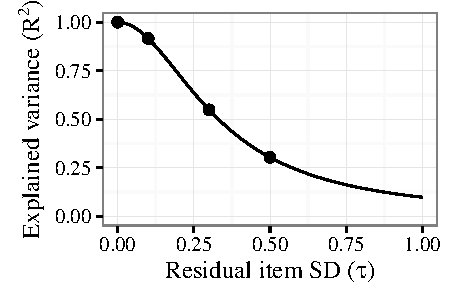
\includegraphics[height=3.5in, trim = 1mm 1mm 1mm 1mm, clip=true]
		{chapter_2/figs/rsq_vs_tau.pdf}
	\caption{$R^2$ versus $\tau$ for the simulations. The points indicate generating values of $\tau$.}
	\label{fig:rsq-vs-tau}
\end{figure}

In summary, three factors are varied between simulation conditions in a crossed design: $\tau$ (and by extention, $R^2$), $I$, and $P$. All other elements are fixed across conditions. Because cross-validation features prominently in this chapter, multiple datasets are simulated within each replication. A ``training'' dataset is created as described above, and along with it three ``test'' datasets are formed: one representing a sample with new items (corresponding to new draws of $\epsilon_i$), one representing a sample with new persons (new draws of $\zeta_p$), and the last representing a sample with both new items and new persons.


\subsection{Models}

Three models, differing only in specification of $\delta_i$, are fit. Model 1 includes only the ``main effects'' for the item covariates:
\begin{equation}
\delta_i^{(1)} = x_{1i}\beta_1 + x_{2i}\beta_2 + x_{3i}\beta_3 + x_{4i}\beta_4
.\end{equation}
Model 2 adds an interaction:
\begin{equation}
\delta_i^{(2)} = x_{1i}\beta_1 + x_{2i}\beta_2 + x_{3i}\beta_3 + x_{4i}\beta_4
+ x_{2i}x_{3i}\beta_5
.\end{equation}
Model 3 adds an additional (spurious \comment{find a better word}) interaction:
\begin{equation}
\delta_i^{(3)} = x_{1i}\beta_1 + x_{2i}\beta_2 + x_{3i}\beta_3 + x_{4i}\beta_4
+ x_{2i}x_{3i}\beta_5 + x_{3i}x_{4i}\beta_6
.\end{equation}
None of the analysis models includes the residual $\epsilon_i$. Each analysis model models ability as in Equations~\ref{eq:theta} and \ref{eq:zeta}. %When $\tau = 0$ is used to generate the data, Model 2 is the true model. Otherwise, none of three match the data generating model.


\section{Naive cross-validation methods}

One naive approach to model selection is the use of significance testing for parameters. In order to select among the three analysis models, a researcher may fit Model~2 and make a judgment based on the p-value for $\beta_5$, the parameter associated with the interaction. If non-significant, the researcher may select Model~1. Otherwise, the researcher may fit Model~3. If the additional interaction ($\beta_6$) is significant, Model~3 would be selected. Otherwise, Model~2 would be selected. This is a forward stepwise procedure.

Figure~\ref{fig:pcheck-bar} presents the proportion of times each model was selected across conditions (combination of $I$, $P$, and $\tau$) when selection is performed via p-values. Within each condition, 200 replications are performed. This method works well when $\tau$ is small but poorly otherwise, and this trend is similar for all combinations of $P$ and $I$. When $\tau = 0$, Model~2 matches the data generating model exactly, and Models~1 and 3 are close. The result is that the correlated nature of responses within an item cluster are appropriately accounted for, yielding correct standard errors for $\mathbf{\beta}$. The preceding is approximately true for small values of $\tau$ like $\tau = .1$. However, with greater values of $\tau$, the analysis models fail to account for the within-cluster dependency, resulting in standard errors that are too low. This shortcoming leads to Model~3 being selected the majority of the time when $\tau$ takes medium to large values.

\begin{figure}[htbp]
	\centering
	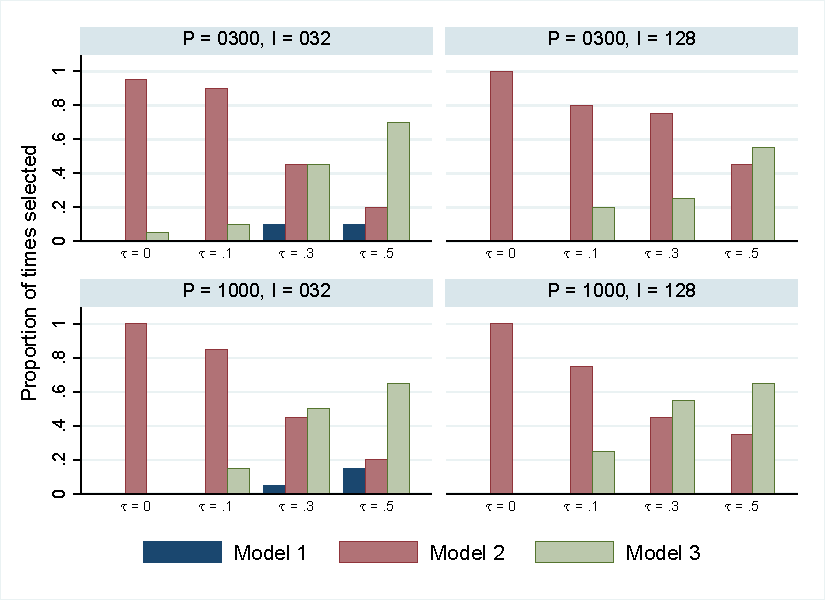
\includegraphics[height=3.5in, trim = 1mm 1mm 1mm 1mm, clip=true]
	{chapter_2/figs/p_pcheck.pdf}
	\caption{Proportion of times each model was selected using significance tests.}
	\label{fig:pcheck-bar}
\end{figure}

Adding item residuals $\epsilon_i$ to the analysis models would provide correct standard errors and p-values. Such a model is prohibitively difficult to fit without resorting to Monte Carlo methods, though. Further, in practical application there may be many more than three models under consideration, which brings up complexities around multiple hypothesis testing. For this reason an appealing alternative is AIC, defined as
\begin{equation}
	\mathrm{AIC} = \mathrm{deviance} + 2k
,\end{equation}
where $k$ is the number of model parameters. The model with the lowest value of AIC is selected. The results of using AIC with the simulated datasets are presented in Figure~\ref{fig:aic-bar}. These results follow similar patterns as for selection by p-values, though a bit worse.

\begin{figure}[htbp]
	\centering
	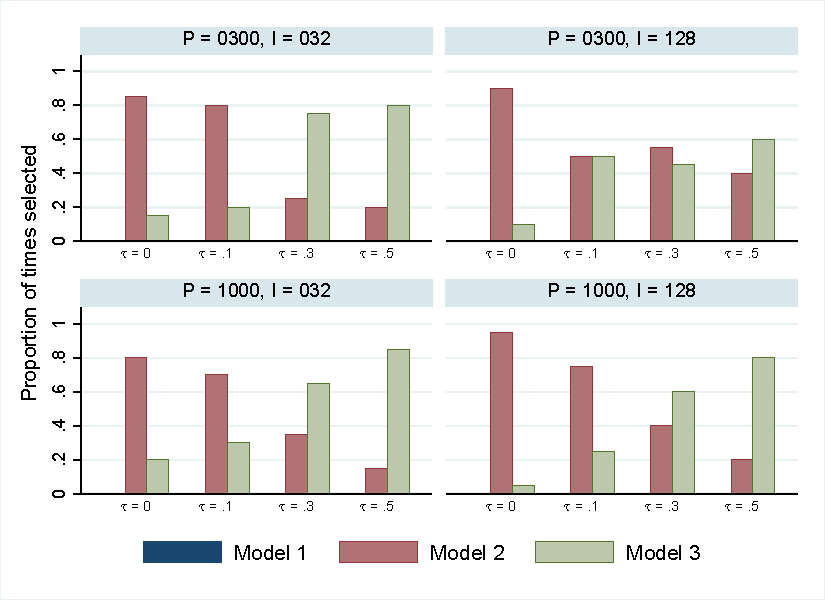
\includegraphics[height=3.5in, trim = 1mm 1mm 1mm 1mm, clip=true]
		{chapter_2/figs/p_aic.pdf}
	\caption{Proportion of times each model was selected using AIC.}
	\label{fig:aic-bar}
\end{figure}

AIC is an approximation for holdout cross-validation, in which a model is estimated using a ``training'' dataset and then evaluated on a ``test'' dataset. In this instance, AIC approximates the deviance that would result from applying the trained model to a test dataset consisting of new persons and the same items. Figure~\ref{fig:person-bar} provides results for the selection procedure using this form of holdout cross-validation. This method performs worse across all conditions than AIC.

\begin{figure}[htbp]
	\centering
	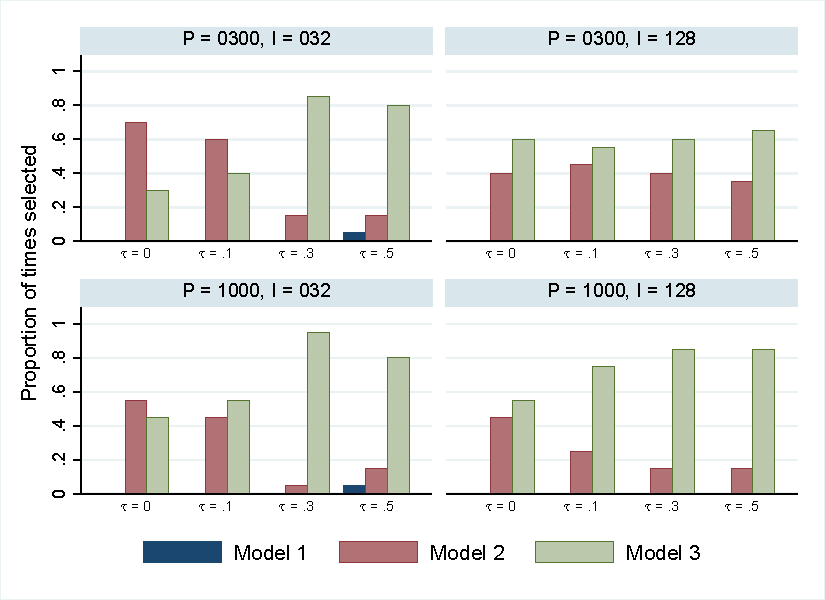
\includegraphics[height=3.5in, trim = 1mm 1mm 1mm 1mm, clip=true]
		{chapter_2/figs/p_new_person_same_item.pdf}
	\caption{Proportion of times each model was selected using holdout cross-validation with holdout data consisting of new persons and the same items.}
	\label{fig:person-bar}
\end{figure}


%\section{Approximation via linear regression}
%
%In the first analysis, sets of item difficulties $\delta_i$ are simulated and regressed on differing sets of item predictors. The item difficulties are treated as known quantities, approximating the situation in which a large number of a persons are available to estimate item parameters to a high degree of accuracy. The simulated datasets do not include persons or responses, only the $I$ values for $\delta_i$ and the item predictors. 
%
%500 replications are preformed for each combination of $I$ and $\tau$. In each, a ``training'' dataset and a ``holdout'' dataset are created. These have differing values of $\delta_i$, owing to having different item residuals, but the structural part is the same between the two. Three linear regression models are fit to each training dataset. Model 1 includes only the ``main effects'' for the item covariates:
%\begin{equation}
%	\delta_i = x_{1i}\beta_1 + x_{2i}\beta_2 + x_{3i}\beta_3 + x_{4i}\beta_4 + \epsilon_i
%.\end{equation}
%Model 2 adds the interaction included in the generating model:
%\begin{equation}
%	\delta_i = x_{1i}\beta_1 + x_{2i}\beta_2 + x_{3i}\beta_3 + x_{4i}\beta_4
%	+ x_{2i}x_{3i}\beta_5 + \epsilon_i
%.\end{equation}
%Model 3 adds an additional (spurious \comment{find better word}) interaction:
%\begin{equation}
%	\delta_i = x_{1i}\beta_1 + x_{2i}\beta_2 + x_{3i}\beta_3 + x_{4i}\beta_4
%	+ x_{2i}x_{3i}\beta_5 + x_{3i}x_{4i}\beta_6 + \epsilon_i
%.\end{equation}
%The fitted models are used to generate predictions for item difficulties in the holdout data, $\hat \delta_{i'}$. They are evaluated with the residual sum of squares:
%\begin{equation}
%	\mathrm{rss} = \sum_{i' = 1}^I (\hat \delta_{i'} - \delta_{i'})^2
%.\end{equation}
%The model with the lowest value of $\mathrm{rss}$ is selected.
%
%Figure~\ref{fig:ols-bar} provides the proportion of times each model was selected for varying values of $I$ and $\tau$. Figure~\ref{fig:ols-line} shows the same but in a pairwise comparison; the blue lines with circular points indicate the proportion of times Model~1 is favored over Model~2, and the green lines with triangular points indicates the proportion of times Model~3 is preferred over Model~2.
%
%\begin{figure}[h]
%	\centering
%	\includegraphics[height=3.5in, trim = 1mm 1mm 1mm 1mm, clip=true]
%		{chapter_2/figs/ols_bar.pdf}
%	\caption{Proportion of times each model was selected (OLS).}
%	\label{fig:ols-bar}
%\end{figure}
%
%\begin{figure}[h]
%	\centering
%	\includegraphics[height=3.5in, trim = 1mm 1mm 1mm 1mm, clip=true]
%		{chapter_2/figs/ols_line.pdf}
%	\caption{Pairwise comparison of selection proportions (OLS).}
%	\label{fig:ols-line}
%\end{figure}


\section{Holdout cross-validation for item predictors}

If the focus of model selection is the choice of item predictors, cross-validation schemes based on test data with the same items are wrongheaded. A useful approach instead is to consider how the item predictors will fare for a new set of items constructed from the same item design. To this end, the analysis models are fit to a training dataset and then evaluated on a holdout dataset representing new persons and new items. Figure~\ref{fig:both-bar} provides the proportion of times each model was selected using this scheme. Across all conditions, Model~2 is selected the majority of times. For $I=32$ items, larger values of $\tau$ are associated with a lower selection proportion for Model~2, while this trend is mitigated when $I=128$.

\begin{figure}[htbp]
	\centering
	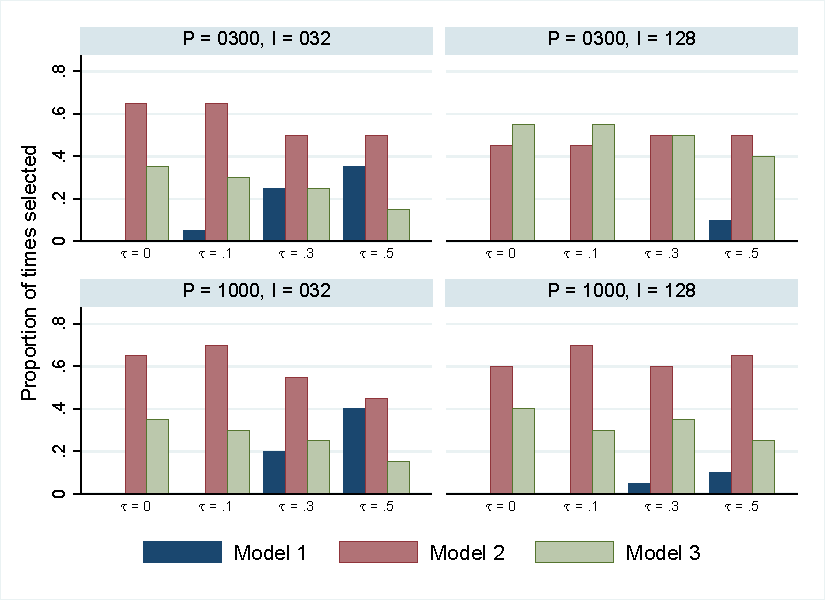
\includegraphics[height=3.5in, trim = 1mm 1mm 1mm 1mm, clip=true]
		{chapter_2/figs/p_new_person_new_item.pdf}
	\caption{Proportion of times each model was selected using holdout cross-validation with holdout data consisting of new persons and new items.}
	\label{fig:both-bar}
\end{figure}

In Figure~\ref{fig:both-line} the results are broken down into pairwise comparisons: Model~1 versus Model~1 and Model~3 versus Model~2. This allows for a closer look at how Models~1 and 3 interfere with the selection of Model~2. Model~1 is selected most often over Model~2 when $\tau$ is large, and this relationship is mitigated when the number of items is large. Model~3 is selected over Model~2 with some frequency, though there is no clear relationship between selection of Model~3 over Model~2 and the simulation conditions.

\begin{figure}[htbp]
	\centering
	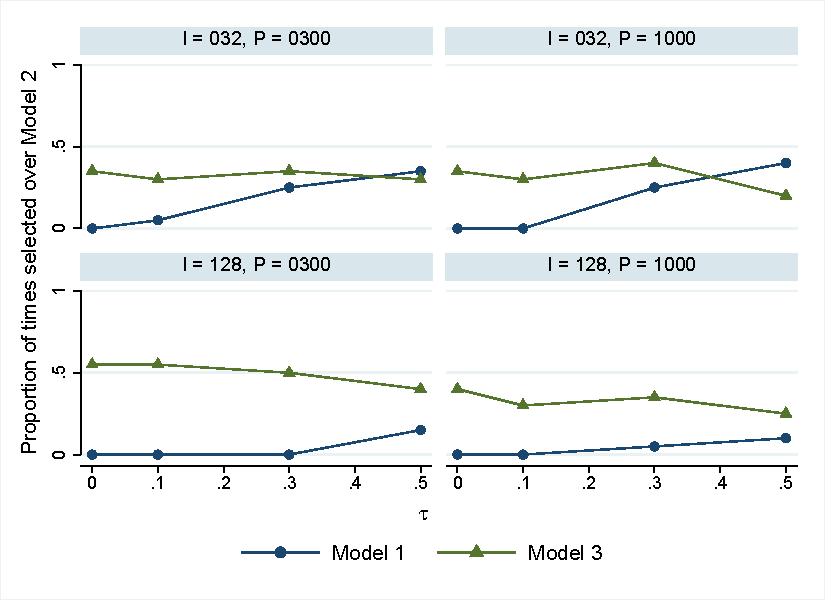
\includegraphics[height=3.5in, trim = 1mm 1mm 1mm 1mm, clip=true]
		{chapter_2/figs/both_line.pdf}
	\caption{Pairwise comparison of selection proportions using holdout cross-validation with holdout data consisting of new persons and new items.}
	\label{fig:both-line}
\end{figure}


\section{Approximations for a single dataset}


\section{Discussion}



%\bibliographystyle{apacite}
%\bibliography{../../Documents/References/references}

\end{document}


